\chapter{基于web可视化工具概述}
\chaptermark{基于web可视化工具概述}
	%GBrowse
	\section{GBrowse}
		\subsection{概述}
		GBrowse是基因组浏览器(GenomeBrowse)的缩写。它是一种基于WEB服务的应用程序,用来可视化基因组的注释及基因性态等其他信息。GBrowse拥有通用模式的便捷和自定义模式的灵活性,用户可以通过网页浏览基因组可视化信息,可以通过搜索功能查找特定基因组,对于查看区域的基因组可以通过缩放进行更加有效的查看,同时提供对基因组相应序列数据的下载,支持gff3,fasta等格式的数据下载。现在GBrowse已经有多个版本,GBrowse1.X版本在2002年就已经开始使用,经过将近十年的发展,各方面都较为成熟,性能比较稳定。GBrowse2.0版本在原有的版本上进行了重写,使用了AJAX技术可以进行动态更新,拥有更好的用户体验,同时对于服务端的性能有了部分的提升。同时GBrowse作为基于web服务的浏览器不用安装,无需进行繁琐的软件配置,用户只需要通过网页浏览器连接到 Internet 就可以使用,对用户个人PC 的要求不高,而且由于数据存储在服务器端,所以用户本地电脑不用消耗太多存储空间来贮放数据。
		\subsection{可视化方式}
		GBrowse用 track的方式进行可视化相关基因组信息,通过对track进行缩放进行细化展示基因跨度可以展示基因组整体效果。GBrowse附带了一个大型字形库,包括饼图,点图,直方图和适用于定量数据的XY图,以及描述序列和序列注释的预期字形数组。通过合理地配置及编码可以实现基因组基因的可视化。
		\subsection{可视化内容}
		GBrowse可视化内容由可视化图谱进行具体显示,可视化图谱可以分为三个部分:overview(概述),region(区域),details(细节)。
		\begin{itemize}
			\item  overview(概述)显示基因组背景,通常是整个组装的染色体或序列组合的大部分,例如支架或重叠群。
			\item region(区域)显示感兴趣区域周围的一部分基因组。
			\item details(细节)显示与概览选择矩形相对应的基因组的放大视图。细节区域包含一个或多个轨迹,显示已经放置在基因组上的注释和其他特征。详细视图由从显示器的一端水平延伸到另一端的多个不同的轨迹组成。每个轨道对应于不同类型的基因组特征,并且通过独特的图形形状和颜色来区分。如图一所示,可以明确地看到。
		\end{itemize}
	GBrowse从版本2.0开始,通过提供直接显示SAM和BAM序列对齐文件,GBrowse支持下一代排序(NGS)数据。SAM/BAM轨道提供语义缩放,并支持本地和远程数据源。可以上传的格式有GFF3,SAM/BAM等多种数据格式的文件。
		\begin{figure}
			\centering
			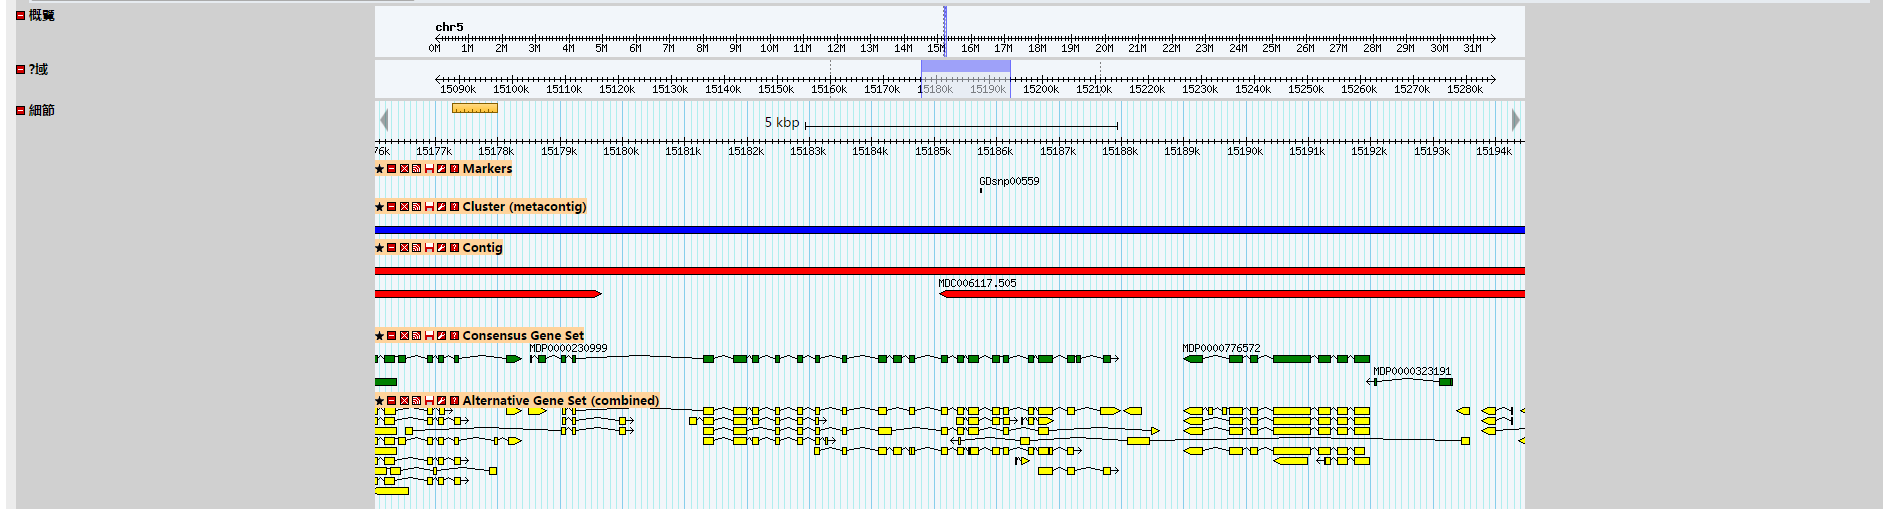
\includegraphics[width = .9\textwidth]{2-1.png}
			\caption{GBrowse页面内容展示图}
		\end{figure}	
		\subsection{系统架构}
		GBrowse是一个Web应用程序,可分为Web服务器端和Web浏览器客户端。GBrowse的服务器端是用Perl编写,部分核心工能由C代码来实现,以达到高性能的需求。服务器端管理一系列包含基因组注释信息的数据库,从Web浏览器接收用户对感兴趣可视化基因区域的请求,并将这些区域显示为PNG,SVG或PDF图像等高清图像返回给Web浏览器端。在Web浏览器端,一系列由Javascript编写的功能函数处理用户界面,实现了跨基因组平移和缩放,通过点击拖动选择一个区域,通过弹出菜单配置曲目并上传曲目数据。\\
		\indent GBrowse的组成可以分成多个部分;顶层是由GBrowse中的CGI模块构成,用来与web服务器进行交互,通过接收用户的相关操作信息,将反馈相关数据给web服务器,在由web服务器将数据返回到用户浏览器,完成用户与服务器之间的交互,同时GBrowse接受第三方扩展,方便对其进行功能扩展。中间层是有PERL库中Bio::Graphics模块与PerlBio模块组成,中间层是GBrowse的核心层,其实现了数据库和用户接口的交互,它将数据库与用户接口进行分离,抽象了数据库连接模块,避免了不同数据库下数据格式存在差异性及连接不兼容的细节问题,从而使得从不同的数据库中读取数据后采用相同数据格式进行显示而且支持多种数据的使用。该模块可以存储jpeg、wbmp、png等不同格式图片并将其转换统一显示到浏览器端。底层是由GBrowse可以使用的数据库类型组成,目前支持MySQL,SQLite,BerkeleyDB等数据库,这种设计可以让GBrowse对大多数主流数据库支持良好,设计者只需编写一个相应的数据库适配器,便可通过该程序将数据导入库模块。\\
		\indent GBrowse支持广泛的基因组数据库和视图是GBrowse最灵活的功能之一。一系列数据适配器扩展允许GBrowse将数据加载到内存,同时支持大型SQL和NoSQL数据库文件及远程数据源和专门的文件格式(如BAM对齐文件)。基因组特征可以由大量可重复使用的“字形”(即feature大致为75个)代表,其范围从通用有色盒子到SNP单倍型区段之间的连锁不平衡的高度特异性表示。
		\begin{figure}[!ht]
			\centering
			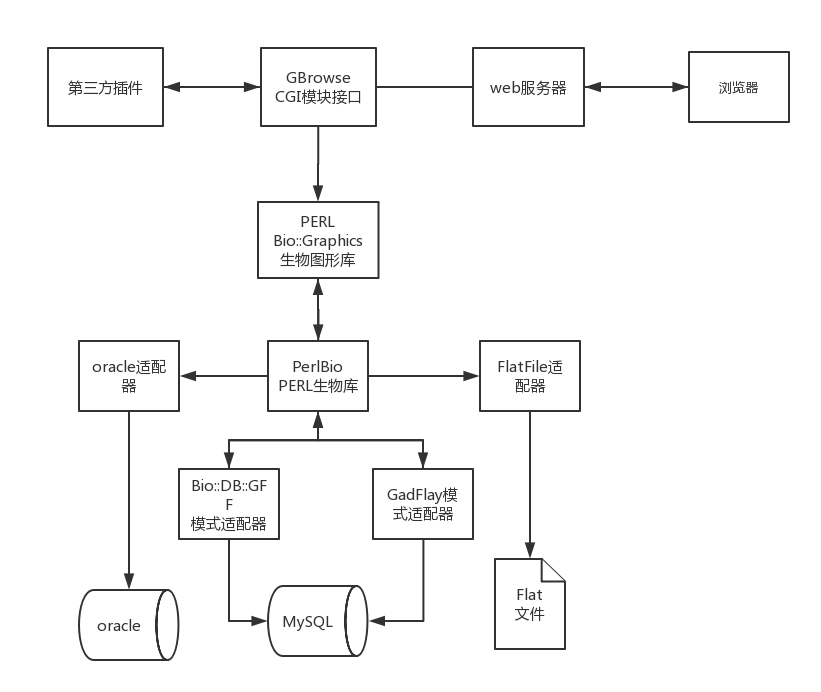
\includegraphics[width = .6\textwidth]{2-2.png}
			\caption{GBrowse系统结构}
		\end{figure}
		\subsection{运行机理}
		当用户向GBrowse发出浏览数据请求时,浏览器根据URL或者AJAX向服务器发送用户请求,服务器接收到用户请求,判断是不是一个静态文件请求,若不是则判断是不是一个CGI可执行文件请求,若是将请求交给GBrowse的CGI扩展,并执行相应的Perl脚本,执行完脚本GBrowse的CGI模块将产生的数据返回给Web服务器,Web服务器接收到数据后再将数据返回给浏览器,触发浏览器端的脚本文件执行使浏览器重新渲染Web页面产生可视化效果。如图2-3GBrowse的CGI模块请求处理流程。
			\begin{figure}[!ht]
				\centering
				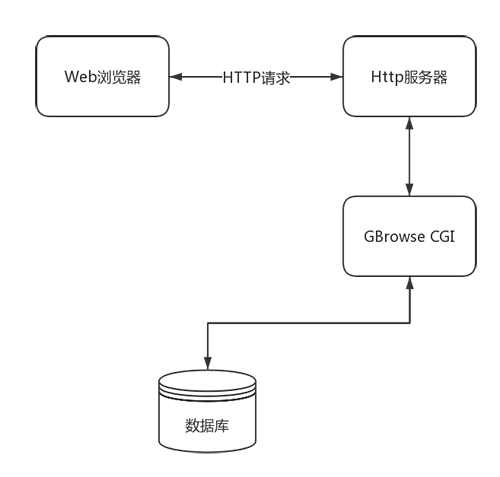
\includegraphics[width = .5\textwidth]{2-3.png}
				\caption{GBrowse模块请求处理}
			\end{figure}
		\subsection{优缺点}
		优点:GBrowse支持大部分基因组数据集格式,对于浏览器的兼容性良好,可以友好的显示在web端,并且拥有良好的跨平台性和兼容性;GBrowse可视化方式多种多样,支持用户上传数据,支持用户管理功能。\\
		\indent 缺点:GBrowse需要许多第三方库。特别是,为了显示NGS测序数据,GBrowse需要Samtools和BigWig库。由于这些依赖关系的安装对于初次安装者来说可能是迷茫且令人困惑的,容易使安装者无法准确地定位出错信息,无法很好地解决环境安装和依赖管理的问题。同时GBrowse2.0作为新开源的基因组可视化工具,存在着部分问题,不适宜新手进行安装使用。针对性能和用户体验方面,GBrowse的大部分工作依赖于服务器端地处理,对服务器端地性能要求过高;用户在通过GBrowse进行基因可视化对比查看时,当需要放大缩小即进行其它操作时,GBrowse会向服务端进行请求,延长用户等待时间,具有较差的用户体验。
		%JBrowse
	\section{JBrowse}
		\subsection{概述}
		JBrowse是一个开源的便携式的基于JavaScript的基因组浏览器,并以GBrowse继任者为目标。它运行速度非常快并且支持大型数据集。JBrowse完全由JavaScript和HTML5构建的,几乎所有的工作,发生在用户的Web浏览器端,对服务器有最低的要求。事实上,JBrowse没有后端服务器代码,后端只是用于格式化数据文件并通过HTTP请求将数据传输到浏览器端。JBrowse可以快速,平滑滚动和缩放,支持缩放多基因组和基因组的深度覆盖测序。 JBrowse具有高度的可扩展插件架构,可以很方便地嵌入任何Web应用中。JBrowse具有良好的跨平台性,目前JBrowse在Electron跨平台应用开发框架下逐步推出Windows等操作系统下的应用软件,方便用户可视化数据。
		\subsection{可视化方式}
		JBrowse用 track 的方式进行可视化,提供平滑的动态移动和缩放功能,也有导航和通道的选择。JBrowse可以展示多种 track 视图,除基本视图外,还可以显示非翻译区、外显子、内含子结构等。
		
		\subsection{可视化内容}
		JBrowse可以展示基因组整体视图,也可以细化展示基因跨度、tRNA、转座子、寡核苷酸、蛋白质结合位点、增强子、基因调控区域、非编码RNA、点突变、序列变异信息等其它基因信息。用户可以自己上传需要可视化的内容的相关基因数据,支持GFF、GFF3、WIG、BED、FASTA、Wiggle、BigWig、BAM 等多种格式的数据文件。如图2-5所示
		\begin{figure}[!ht]
			\centering
			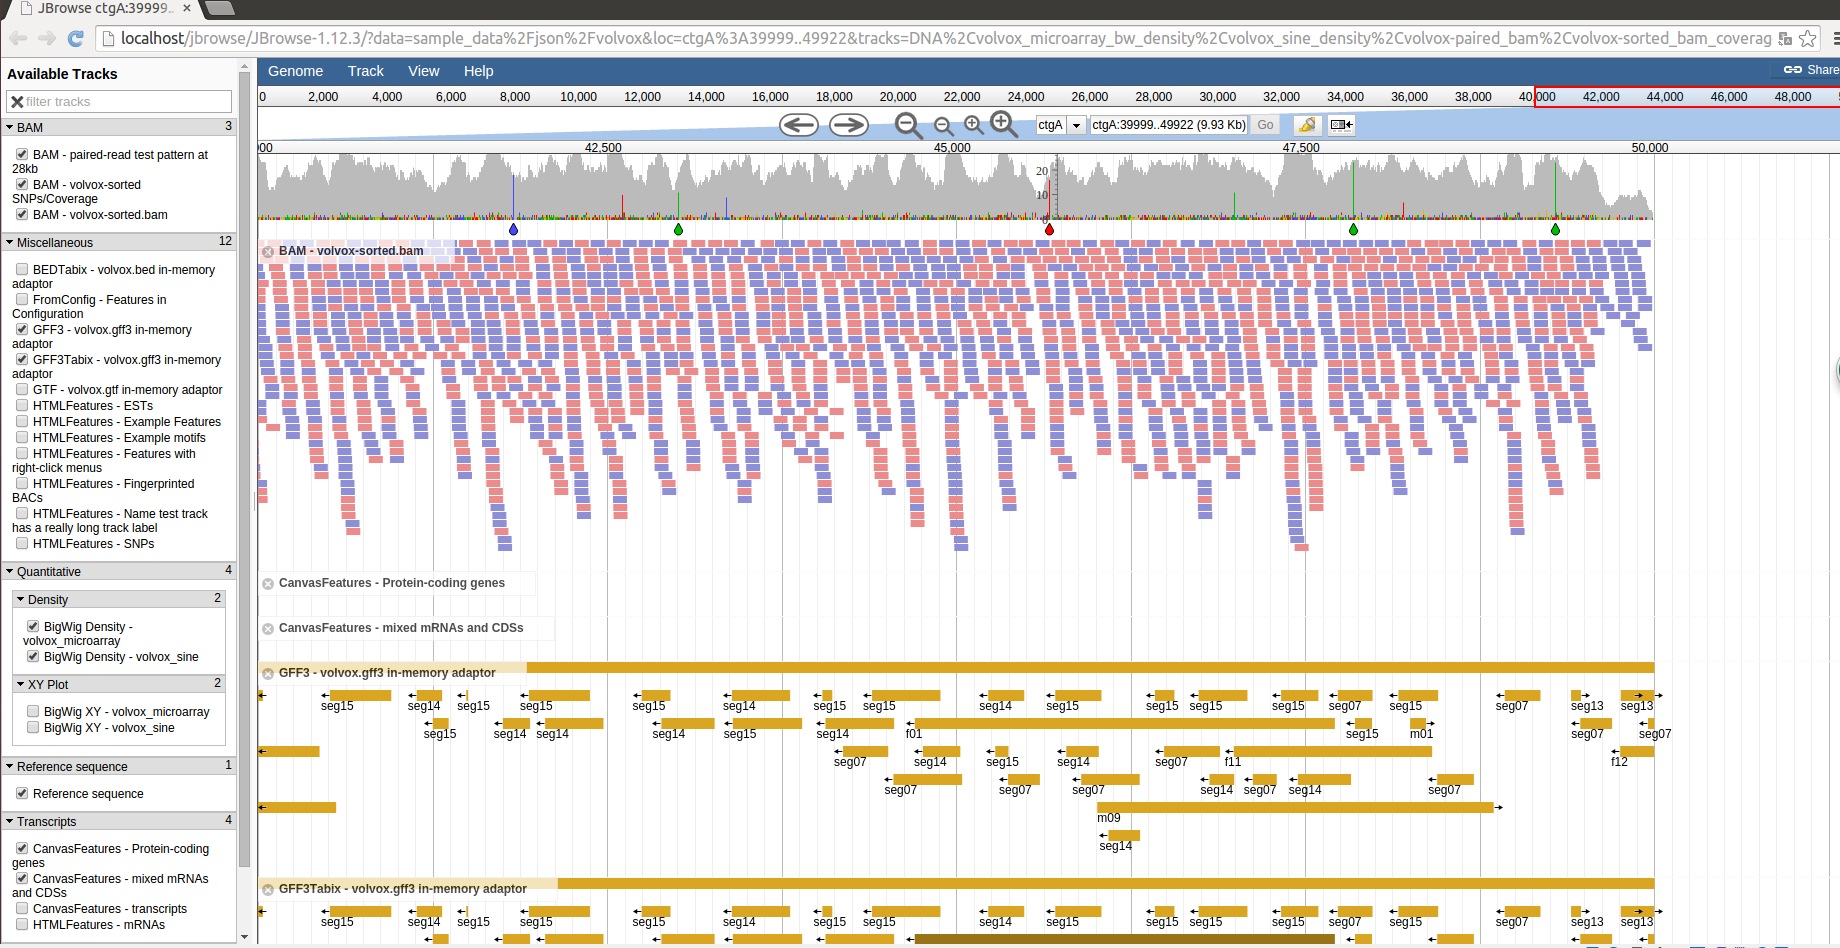
\includegraphics[width = .6\textwidth]{2-4.png}
			\caption{JBrowse可视化内容}
		\end{figure}
		\subsection{系统架构}
		JBrowse 完全由Javascript和 HTML5构建实现,对外提供 Javascript API功能接口,后端数据通过Perl工具进行处理。Web端对浏览器的要求是需要支持 HTML5 中的新标签(如 Canvas),目前主流的浏览器支持良好;后台服务器端主要采用 Json文件进行数据存储。  Json作为一种轻量级的数据交换格式,是基于Javascript语言规范进行设计,属于 Javascript的一个子集,在Javascript中的以对象和数组的形式存在,因此可以实现较快的前后台通信,提高通信速度加强用户体验。如图2-5所示,JBrowse分为前端和后端;在后端JBrowse可以分为三部分,数据库适配器,配置文件,数据管理工具支持多种数据适配器的支持比如Bio::DB::SeqFeature::Store
		\begin{figure}[!ht]
			\centering
			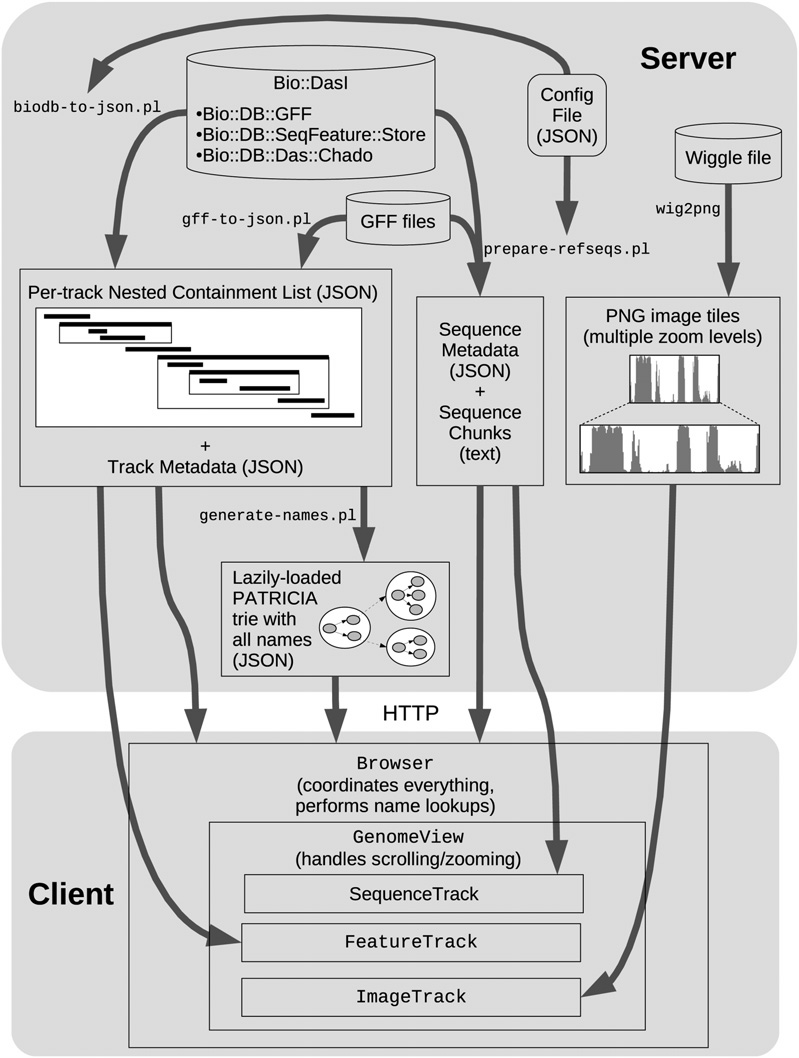
\includegraphics[width = .6\textwidth]{2-5.png}
			\caption{JBrowse系统架构}
		\end{figure}
		\subsection{运行机理}
		
		\subsection{优缺点}
		优点:JBrowse 属于新一代基因组浏览器,作为GBrowse的继任者,是基于最新的前端技术开发的。在 JBrowse 中,服务器端的负荷极大地降低,后台服务器只需要向浏览器客户端发送数据文件,将繁杂的计算工作从服务端脱离出来,大量计算工作被合理分配到了前端。同时,JBrowse对Cookies技术也得到了很好的支持,可以有效记录用户的喜好。\\
		\indent 缺点: JBrowse 把可视化主要工作放在了浏览器端,但其可视化方法仅是一些普通的HTML 标签实现,造成可视化不友好等问题。同时浏览器在绘制图像时需要运行大量的JavaScript代码,而且目前主流浏览器对 HTML5 中新标签的支持不完善,造成用户体验不佳等问题。
		